\chapter{Practice: A WSN with XBee's AT mode}\label{ATSensorNetwork}
\section*{Suggested read: Chapers~\ref{introToXBee},~\ref{pract:simpleChat} and~\ref{pract:thermometer}}

In this assignment we will build a sensor network using the AT (as opposed to the API) mode.
This means that we will directly write characters in one end and read them at the other end.
We can replace any of the two ends by a serial terminal emulation (\emph{\color{blue}{\href{http://en.wikipedia.org/wiki/Minicom}{minicom}}}).

We start by flashing two XBees using X-CTU.
We will install the AT firmware in them.
One has to be the coordinator and the other the router.

Then we have to configure the PANID, and the destination address for each of them.
The configuration can be done using X-CTU or the minicom.
Verify the configuration observing the RSSI LED and then connecting minicom to both XBee and sending information from one XBee to the other as in the chat assignment (see Chapter~\ref{pract:simpleChat}).

We will use one of the XBees on the solderless breadboard, connected to the Arduino.
As usual, use the Arduino 3.3V to power the breadboard and connect the serial pins of the XBee to the Arduino.
Use the breadboard to install your light or temperature sensors and connect them to the analog inputs of the Arduino. You can take a look at Chapter~\ref{pract:thermometer} to ease your way through this task. Figure~\ref{fig:thermometerInArduino} provides the necessary connections.

\begin{figure}[htbp]
  \centering
  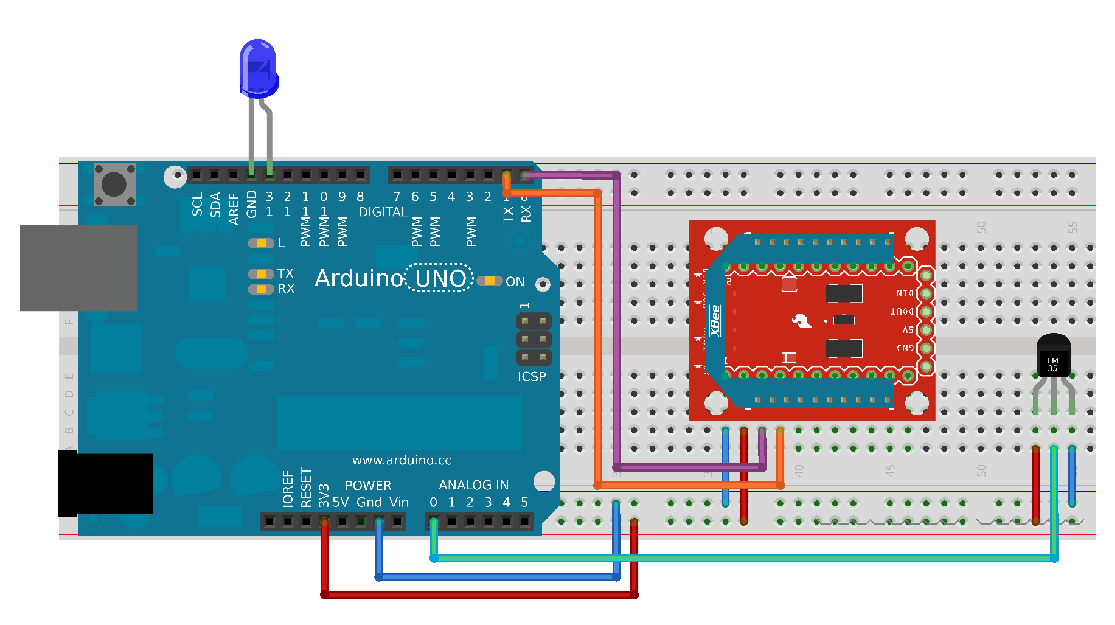
\includegraphics[width=0.85\linewidth]{figures/thermometerInArduino.eps}
  \caption{Thermometer and XBee transmitter.}
  \label{fig:thermometerInArduino}
\end{figure}

Use the example code in Listing \ref{code:ATWSN-router} as a reference to read data from the sensors and send it using the serial connection from the Arduino to the XBee. 
Then the XBee will automatically send it to the remote XBee.
Note that in the code we include identifiers for the node and sensor.

\begin{lstlisting} [caption = {Reading from analog input and sending the data via the XBee.}, language = C, label = {code:ATWSN-router}, numbers = left, escapeinside={@}{@}]
int ledPin = 13;

void setup()
{
  pinMode(ledPin, OUTPUT);
  Serial.begin(9600);
}

void loop()
{
  digitalWrite(ledPin, HIGH);
  delay(1000);
  digitalWrite(ledPin, LOW);
  delay(1000);
  Serial.print("N "); //node
  Serial.print("10 ");
  Serial.print("S "); //sensor
  Serial.print("1 ");
  Serial.print("T ");
  Serial.println(analogRead(A0));
}
\end{lstlisting}


The other XBee will be connected directly to the computer.
This will be the sink and will gather the sensed data.
We will program this part in Python using the Listing \ref{code:ATWSN-sink} for reference.


\begin{lstlisting} [caption = {Simple code that reads the message that arrive to the XBee in AT mode.}, language = Python, label = {code:ATWSN-sink}, numbers = left, escapeinside={@}{@}]

# Derived from code by Alejandro Andreu
import serial
import time
import sys
import shlex
from time import gmtime, strftime

print 'Receiving data in transparent mode'

def main():
    if len(sys.argv) is 1:
        print 'You must provide the path to the serial port as an argument, for instance: "python <code.py> /dev/ttyUSB0".'
        sys.exit()
    portname = sys.argv[1]
    try:
        with open(portname) as f: pass
    except IOError as e:
        print e, '\n'
        sys.exit()

    s = serial.Serial(portname, 9600)

    print 'Opened'

    while 1:
        received = s.readline()
        print "Received at: ", strftime("%d-%m-%Y %H:%M:%S",gmtime()),": ", received
        #splitted = shlex.split(received)
        #for i in range(len(splitted)):
        #    print splitted[i]
        time.sleep(1)

if __name__ == "__main__":
    main()
\end{lstlisting}

Now we can collaborate with other groups to build larger networks and do more interesting stuff.
For example
\begin{itemize}
\item Compute time averages, geographical averages and time-geographical averages.
\item Use EWMA or other filters for time average.
\item Create alarms that use a combination of the data received from different sensors and nodes. 
For example, if the majority of nodes report light and temperature readings, trigger a fire alarm.
\item The alarm can be an LED on the Arduinos.
Use broadcast addresses if you want to reach all the nodes in the PANID.
\end{itemize}
